\documentclass[aspectratio=169]{beamer}
\usepackage{tikz}
\usepackage{amsmath,amssymb,amsfonts}
\usepackage{mathtools}
\usepackage{xcolor}
\usepackage{tikz}
\usetikzlibrary{arrows.meta, positioning}
\usetikzlibrary{arrows.meta, angles, quotes, positioning}
\usepackage{graphicx}
\usepackage{booktabs}
\usepackage{hyperref}
\usepackage{bm}
\definecolor{darkgreen}{rgb}{0.0, 0.5, 0.0}
% Custom commands
\newcommand{\RR}{\mathbb{R}}
\DeclareMathOperator{\tr}{tr}

% Beamer theme
\usetheme{Madrid}
\usecolortheme{default}
\setbeamertemplate{navigation symbols}{}
\setbeamertemplate{footline}[frame number]
\AtBeginSection{
	\begin{frame}{Outline}
		\tableofcontents[currentsection]
	\end{frame}
}
\title{Origin, Dilemma and Development of the DFP Algorithm}
\author{Huicong Chen\\
Sun Yat-sen University}
\date{\today}

\begin{document}
	
	% ========== Title Slide ==========
	\begin{frame}
		\titlepage
	\end{frame}
	
	% ========== Outline ==========
	\begin{frame}{Outline}
		\tableofcontents
	\end{frame}
	
	% ========== Section 1: Introduction ==========
	\section{Introduction to the DFP Algorithm}
	
	\begin{frame}{Motivation}
		\begin{block}{unconstrained optimization}
			\[
			\min_{x\in\RR^n} f(x), \qquad f\in C^2(\RR^n)
			\]
		\end{block}
		
		\textbf{Newton's method:}
		\[
		x_{k+1}=x_k-[\nabla^2 f(x_k)]^{-1}\nabla f(x_k)
		\]
		\begin{itemize}
			\item \textbf{Pros:} Quadratic convergence near the solution.
			\item \textbf{Cons:} Computing $\nabla^2 f(x_k)$ costs $O(n^2)$; inversion $O(n^3)$.
		\end{itemize}
		
		Quasi-Newton idea: Replace Hessian by an approximation $B_k$ built \emph{only from gradient information}.
	\end{frame}
	
	\begin{frame}{The First Quasi-Newton Method: DFP}
		\begin{itemize}
			\item \textbf{1959:} Davidon\footnote{Davidon, W. C., \emph{Variable metric method for minimization}, SIAM J. Optim., 1(1):1–17, 1991.} proposes the first quasi-Newton algorithm (Argonne National Laboratory technical report).
			\item \textbf{1963:} Fletcher \& Powell\footnote{Fletcher, R., Powell, M. J. D., \emph{A rapidly convergent descent method for minimization}, Comput. J., 6(2):163–168, 1963.} systematically revise and popularize it.
		\end{itemize}
		
		The resulting DFP update introduces the secant condition:
		\[
		B_{k+1}s_k = y_k,\quad s_k=x_{k+1}-x_k,\; y_k=g_{k+1}-g_k
		\]
		Where $B_k$ approximates the Hessian and $g_k=\nabla f(x_k)$.
		
	\end{frame}
\begin{frame}{Wolfe Conditions}
	Before discussing the specific algorithm, we first introduce the Wolfe conditions for step length selection.
	
	\begin{columns}[T]
		\begin{column}{0.48\textwidth}
			\textbf{Weak Wolfe conditions:}
			\[
			\begin{aligned}
				f(x_k + \alpha d_k) &\le f(x_k) + c_1 \alpha \nabla f(x_k)^\top d_k\\
				\nabla f(x_k + \alpha d_k)^\top d_k &\ge c_2 \, \nabla f(x_k)^\top d_k
			\end{aligned}
			\]
			where $0 < c_1 < c_2 < 1$ (e.g., $c_1=10^{-4}$, $c_2=0.9$).
			
			\vspace{0.2cm}
			\textbf{Strong Wolfe conditions:} replace curvature with
			\[
			\big| \nabla f(x_k + \alpha d_k)^\top d_k \big| \le -c_2 \, \nabla f(x_k)^\top d_k.
			\]
		\end{column}
		
		\begin{column}{0.48\textwidth}
			\begin{center}
				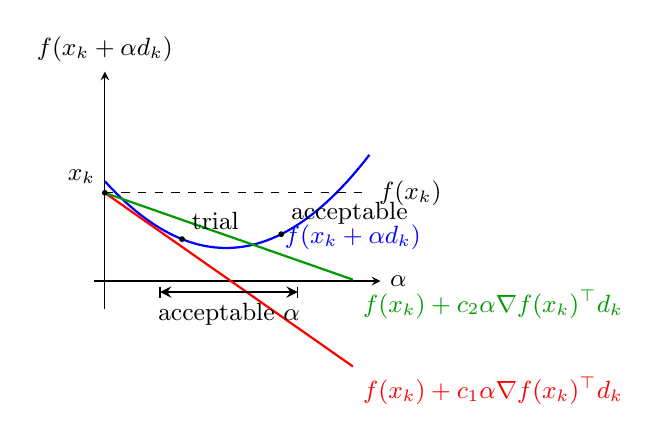
\begin{tikzpicture}[scale=0.7, >=stealth, font=\small]
					% Axes
					\draw[->] (-0.2,0) -- (5,0) node[right] {$\alpha$};
					\draw[->] (0,-0.5) -- (0,3.8) node[above] {$f(x_k+\alpha d_k)$};
					
					% Function curve (convex)
					\draw[thick, blue] plot[smooth, domain=0:4.8, samples=100] (\x, {0.25*(\x-2.2)^2 + 0.6});
					
					% f(x_k) horizontal line
					\draw[dashed] (0,1.6) -- (4.8,1.6) node[right] {$f(x_k)$};
					
					% Sufficient decrease line
					\draw[thick, red] (0,1.6) -- (4.5, {1.6 - 0.7*4.5}) node[below right] {$f(x_k) + c_1\alpha\nabla f(x_k)^\top d_k$};
					
					% Curvature condition boundary line
					\draw[thick, green!60!black] (0,1.6) -- (4.5, {1.6 - 0.35*4.5}) node[below right] {$f(x_k) + c_2\alpha\nabla f(x_k)^\top d_k$};
					
					% Mark acceptable interval
					\draw[<->, thick] (1.0, -0.2) -- (3.5, -0.2);
					\draw (1.0, -0.3) -- (1.0, -0.1);
					\draw (3.5, -0.3) -- (3.5, -0.1);
					\node at (2.25, -0.6) {acceptable $\alpha$};
					
					% Labels
					\fill (0,1.6) circle (1.5pt) node[above left] {$x_k$};
					\fill (1.4, {0.25*(1.4-2.2)^2+0.6}) circle (1.5pt) node[above right] {trial};
					\fill (3.2, {0.25*(3.2-2.2)^2+0.6}) circle (1.5pt) node[above right] {acceptable};
					
					\node[blue, below] at (4.5, 1.2) {$f(x_k+\alpha d_k)$};
				\end{tikzpicture}
			\end{center}
		\end{column}
	\end{columns}
\end{frame}
	\begin{frame}{DFP Update}
		\textbf{DFP update:}
		\[
		\boxed{B_{k+1}=B_k - \frac{B_k s_k y_k^\top + y_k s_k^\top B_k}{y_k^\top s_k}
			+ \left(1+\frac{s_k^\top B_k s_k}{y_k^\top s_k}\right)\frac{y_k y_k^\top}{y_k^\top s_k}}
		\]
		
		\vspace{0.2cm}
		\textbf{Key property:}\\
		If $B_k$ is symmetric positive definite and $y_k^\top s_k>0$, then $B_{k+1}$ is also symmetric positive definite.
		\vspace{0.2cm}
		\begin{itemize}
			\item The condition $y_k^\top s_k>0$ is guaranteed by the Wolfe line search (for convex $f$).
			\item Positive definiteness ensures $p_k=-B_k^{-1}g_k$ is a descent direction.
		\end{itemize}
	\end{frame}

	\begin{frame}{The BFGS Method}
		\textbf{BFGS update} (Broyden, Fletcher, Goldfarb, Shanno, 1970)\footnote{Broyden, C. G., \emph{The convergence of a class of double-rank minimization algorithms}, J. Inst. Math. Appl., 6:76–90, 1970.}:
		\[
		B_{k+1}^{\text{BFGS}} = B_k - \frac{B_k s_k s_k^\top B_k}{s_k^\top B_k s_k} + \frac{y_k y_k^\top}{y_k^\top s_k}
		\]
		
		Let \(H_k = B_k^{-1}\). Then the inverse update has the \textbf{same form}:
		\[
		H_{k+1}^{\text{BFGS}} = H_k - \frac{H_k y_k y_k^\top H_k}{y_k^\top H_k y_k} + \frac{s_k s_k^\top}{y_k^\top s_k}
		\]
	\end{frame}
	
	\begin{frame}{The Broyden Family}
		DFP and BFGS belong to a one-parameter family:
		\[
		B_{k+1}(\phi_k) = (1-\phi_k)\, B_{k+1}^{\text{BFGS}} + \phi_k\, B_{k+1}^{\text{DFP}}, \quad \phi_k \in [0,1]
		\]
		\text{or equivalently}
		\[
		B_{k+1} = B_k - \frac{B_k s_k s_k^\top B_k}{s_k^\top B_k s_k} + \frac{y_k y_k^\top}{y_k^\top s_k} + \phi_k (s_k^\top B_k s_k) v_k v_k^\top,
		\]
		where $\displaystyle v_k = \frac{y_k}{y_k^\top s_k} - \frac{B_k s_k}{s_k^\top B_k s_k}$.
		
		\begin{itemize}
			\item $\phi_k = 0$: BFGS
			\item $\phi_k = 1$: DFP
		\end{itemize}
	\end{frame}
	
	% ========== Part 2: Superlinear Convergence ==========
	\section{Superlinear Convergence of the DFP Algorithm}
	
	\begin{frame}{Superlinear Convergence}
		\begin{definition}[Superlinear rate]
			\[
			\lim_{k\to\infty} \frac{\|x_{k+1}-x^*\|}{\|x_k-x^*\|} = 0.
			\]
		\end{definition}
		
		\begin{theorem}[Dennis \& Moré, 1971]\footnotemark
			Let $x_{k+1}=x_k - B_k^{-1}\nabla f(x_k)$ converge to $x^*$ with $\nabla f(x^*)=0$, $\nabla^2 f(x^*)$ nonsingular. Then convergence is superlinear \textbf{if and only if}
			\[
			\lim_{k\to\infty} \frac{\|[B_k - \nabla^2 f(x^*)]\,(x_{k+1}-x_k)\|}{\|x_{k+1}-x_k\|}=0.
			\]
		\end{theorem}
		\footnotetext{Dennis, J. E., Moré, J. J., \emph{A characterization of superlinear convergence and its application to quasi-Newton methods}, Math. Comp., 28:549–560, 1974.}
	\end{frame}
	
	\begin{frame}{Superlinear Convergence Results}
		\begin{itemize}
			\item \textbf{Exact line search (Powell, 1971):}\footnote{Powell, M. J. D., \emph{On the convergence of the variable metric algorithm}, J. Inst. Math. Appl., 7:21–36, 1971.} \\
			For uniformly convex $f$, DFP converges superlinearly.
			
			\item \textbf{Inexact line search (Wolfe conditions, Broyden family):}\footnote{Byrd, R. H., Nocedal, J., Yuan, Y., \emph{Global convergence of a class of quasi-Newton methods on convex problems}, SIAM J. Numer. Anal., 24:1171–1190, 1987.} \\
			All methods in the Broyden family (including DFP) satisfy the Dennis condition and thus converge superlinearly, provided the iterates converge.
		\end{itemize}
	\end{frame}
	
	\section{Global Convergence of the DFP Algorithm}
	
	\begin{frame}{The Course of Global Convergence Research}
		\begin{itemize}
			\item \textbf{1971 (Powell)}\footnote{Powell, 1971.}: DFP with \emph{exact} line search converges globally for convex functions.
			\item \textbf{1976 (Powell)}\footnote{Powell, M. J. D., \emph{Some global convergence properties of a variable metric algorithm for minimization without exact line searches}, in Nonlinear Programming, SIAM-AMS Proceedings, Vol. IX, pp. 53–72, 1976.}: BFGS with \emph{inexact} (Wolfe) line search converges globally.
			\item \textbf{1987 (Byrd, Nocedal \& Yuan)}\footnote{Byrd, Nocedal, Yuan, 1987.}: All convex Broyden family methods converge globally \textbf{except DFP}.
			\item \textbf{1995 (Yuan)}\footnote{Yuan, Y., \emph{On the convergence of DFP algorithm}, Annals of Operations Research, 103:87–99, 2001 (Received 1995).}: Proposes sufficient conditions for DFP with weak Wolfe line search.
			\item \textbf{1995--present:} No definitive resolution for DFP with inexact line search.
		\end{itemize}
	\end{frame}
	
	\begin{frame}{Zoutendijk Condition}
		\begin{theorem}[Zoutendijk, 1970]\footnotemark
			Suppose:
			\begin{itemize}
				\item \(f\) is bounded below and \(\nabla f\) is Lipschitz continuous.
				\item The line search satisfies the \textbf{Wolfe conditions}.
				\item \(p_k\) is a descent direction.
			\end{itemize}
			Then
			\[
			\sum_{k=0}^{\infty} \cos^2\theta_k \;\|\nabla f_k\|^2 \;<\; \infty,
			\]
			where \(\cos\theta_k = \dfrac{-\nabla f_k^\top p_k}{\|\nabla f_k\|\|p_k\|}\).
		\end{theorem}
		\footnotetext{Zoutendijk, G., \emph{Nonlinear programming, computational methods}, in Integer and Nonlinear Programming, J. Abadie, ed., North-Holland, 1970.}
	\end{frame}
	
	\begin{frame}{From Zoutendijk to Trace Control}
		For quasi-Newton methods:
		\[
		p_k = -B_k^{-1}g_k,\quad \cos\theta_k = \frac{g_k^\top B_k^{-1}g_k}{\|g_k\|\,\|B_k^{-1}g_k\|}.
		\]
		
		\textbf{Step 1: Lower bound via eigenvalues.}  
		\[
		\cos\theta_k \;\ge\; \frac{1}{\kappa(B_k)},\qquad 
		\kappa(B_k)=\frac{\lambda_{\max}(B_k)}{\lambda_{\min}(B_k)}.
		\]
		
		\textbf{Step 2: Condition number bounded by traces.}  
		For a positive definite matrix:
		\[
		\kappa(B_k) \;\le\; \operatorname{tr}(B_k)\,\operatorname{tr}(B_k^{-1}).
		\]
		(Since \(\lambda_{\max}\le\operatorname{tr}(B_k)\) and \(1/\lambda_{\min}\le\operatorname{tr}(B_k^{-1})\).)
	\end{frame}
	
	\begin{frame}{Trace Control in the Broyden Family}
		From the Broyden family update\footnote{R.~H. Byrd, J.~Nocedal, Y.-X. Yuan, 1987.}:
		\[
		\operatorname{tr}(B_{k+1}) = \operatorname{tr}(B_k) + \frac{\|y_k\|^2}{y_k^\top s_k}
		+ \phi_k \frac{\|y_k\|^2}{y_k^\top s_k}\frac{s_k^\top B_k s_k}{y_k^\top s_k}
		- (1-\phi_k)\frac{\|B_k s_k\|^2}{s_k^\top B_k s_k}
		- 2\phi_k\frac{y_k^\top B_k s_k}{y_k^\top s_k}.
		\]
		
		\textbf{Crucial term:} 
		\[
		\frac{\|B_k s_k\|^2}{s_k^\top B_k s_k} \ge \frac{\lambda_k}{c_2 \cos^2\theta_k}.
		\]
		And the step lengths satisfy:
		\[
		\prod_{j=1}^k \lambda_j \ge c_4^k,\quad c_4>0.
		\]
		From this, we can prove that all methods in the Broyden family except for DFP are globally convergent.
	\end{frame}
	
	\begin{frame}{Yuan's Framework}
		\textbf{Assumptions:}
		\begin{enumerate}
			\item[(i)] \(f\) is twice continuously differentiable and \textbf{uniformly convex}:
			\[
			\exists\,c_3>0,\quad p^\top\nabla^2 f(x)p \ge c_3\|p\|^2,\quad \forall p,x.
			\]
			\item[(ii)] The line search satisfies the \textbf{weak Wolfe conditions}.
		\end{enumerate}
		
		Under these assumptions, Yuan proved four \textbf{sufficient conditions} for global convergence of DFP\footnote{Yuan, 1995.}.
		\begin{itemize}
			\item $\alpha_k \ge \varepsilon > 0$ and the line search satisfies the \textbf{strong Wolfe conditions}.
			\item $\|g_{k+1}\|_2 \le \|g_k\|_2$ for all sufficiently large $k$ (monotone gradient norm).
			\item $\displaystyle\sum_{k=1}^{\infty} \|s_k\| < \infty$.
		\end{itemize}
	\end{frame}
	
	\begin{frame}{Sufficient Condition 4}
		\begin{theorem}[Yuan, 1995]
			Under uniform convexity and weak Wolfe line search, if
			\[
			y_k^\top B_k g_k \le 0 \quad \text{for all } k,
			\]
			then the DFP algorithm converges globally.
		\end{theorem}
		Yuan proved the following inequality to control the trace of $B_{k+1}^2$:
		\[
		\tr(B_{k+1}^2) \le \tr(B_k^2) + C \frac{1}{\|d_k\|^2}.
		\]
		Then he used it to control $\tr(B_k)$ and prove global convergence.
	\end{frame}
	
	\begin{frame}{Limitations of Yuan's Conditions}
		\begin{itemize}
			\item All four conditions are sufficient for global convergence, but they are difficult to check in practice within the standard DFP framework.
			\item Yuan also proposed two open inequalities:
			\[
			\sum_{i=1}^k \frac{y_i^\top B_i s_i}{s_i^\top y_i} \le c_{12} \sum_{i=1}^k \alpha_i,
			\]
			\[
			\sum_{i=1}^k \left|\frac{y_i^\top B_i^2 s_i}{s_i^\top y_i}\right| \le c_{13} \sum_{i=1}^k \frac{1}{\|d_i\|^2},
			\]
			neither has been proven or disproven.
			\item This reflects that the DFP algorithm's convergence behavior is not ideal – in particular, the step length $\|s_k\|$ is not well controlled.
		\end{itemize}
	\end{frame}
	
	% ========== Part 4: Projection DFP Algorithm ==========
	\section{Improvement of the DFP Algorithm}
	
\begin{frame}{Projection DFP}
	\begin{columns}[T, onlytextwidth]
		% 左侧：文本描述
		\begin{column}{0.48\textwidth}
			Therefore, Yuan, Zhou and Pham\footnotemark[1] modify DFP by projecting the step at out-points to enforce $\sum\|s_k\|<\infty$.
			
			\vspace{1ex}
			Define a constant $\tau>0$ (e.g., $\tau=0.01$) and the set of \textbf{in-points}:
			\[
			\mathcal{PX}_k = \{\, x_k \mid g_k^\top d_k \le -\tau \|d_k\| \,\}.
			\]
			Points not in $\mathcal{PX}_k$ are \textbf{out-points}.
			
			\vspace{1ex}
			For in-points, the iteration points are the same as standard DFP:
			\[
			x_{k+1} = x_k + \alpha_k d_k.
			\]
		\end{column}
		
		% 右侧：示意图
		\begin{column}{0.48\textwidth}
			\centering
			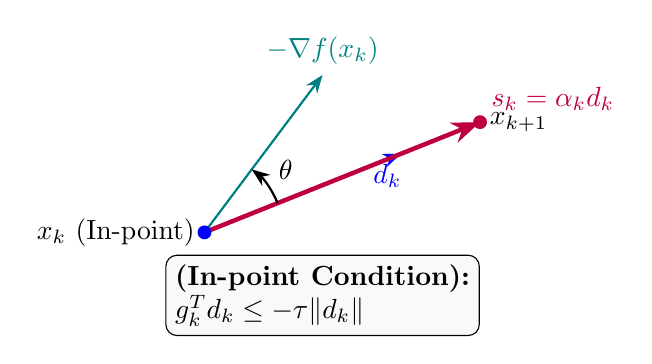
\begin{tikzpicture}[scale=1.0, >=Stealth, baseline=(current bounding box.center)]
				\coordinate (Xk) at (0, 0);                 
				\coordinate (NegGrad) at (1.5, 2.0);       
				\coordinate (Dk_dir) at (2.5, 1.0);         
				\coordinate (Xk1) at (3.5, 1.4);            
				
				\draw[->, thick, teal] (Xk) -- (NegGrad) node[above] {$-\nabla f(x_k)$};
				\draw[->, thick, blue] (Xk) -- (Dk_dir) node[below, xshift=-5pt] {$d_k$};
				\draw[->, ultra thick, purple] (Xk) -- (Xk1) node[above right] {$s_k = \alpha_k d_k$};
				
				\pic [draw, thick, "$\theta$", angle radius=1cm, angle eccentricity=1.3, ->] {angle = Dk_dir--Xk--NegGrad};
				
				\fill[blue] (Xk) circle (2.5pt) node[left, text=black] {$x_k$ (In-point)};
				\fill[purple] (Xk1) circle (2.5pt) node[right, text=black] {$x_{k+1}$};
				
				\node[align=left, draw, fill=gray!5, rounded corners, text=black] at (1.5, -0.8) {
					\textbf{(In-point Condition):}\\
					$g_k^T d_k \le -\tau \|d_k\|$
				};
			\end{tikzpicture}
		\end{column}
	\end{columns}
	
	
	\footnotetext[1]{Yuan, G., Zhou, P., Pham, H. T., \emph{A projection DFP quasi-Newton algorithm and its applications}, Numerical Algorithms, 2026.}
\end{frame}
	\begin{frame}{Projection DFP}
		For an out-point ($x_k \notin \mathcal{PX}_k$), let $\hbar_k = x_k + \alpha_k d_k$.
		
		Define the \textbf{parabolic surface}:
		\[
		\{ x \mid g(\hbar_k)^\top d_k - \sigma_1 g(x)^\top d_k + \sigma_2 \tau \|d_k\| = 0 \},
		\]
		where \( \sigma_1 + \sigma_2 < 1 \) with \( \sigma_1 \in (0, c_2) \) and \( \sigma_2 \in (c_2 - \sigma_1, 1) \) are constants, and \(c_2\) is the parameter in the weak Wolfe conditions.(e.g.,$\sigma_1=0.425,~\sigma_2=0.5,~c_2=0.85$)
		
		The projected iterate is
		\[
		x_{k+1} = x_k + \frac{PP_k}{\|d_k\|}\,\alpha_k d_k,\quad
		PP_k = g(\hbar_k)^\top d_k - \sigma_1 g(x_k)^\top d_k + \sigma_2 \tau \|d_k\|.
		\]
		
		Then $x_{k+1}$ lies on the parabolic surface, and the step is shortened.
	\end{frame}
\begin{frame}{Projection DFP}
	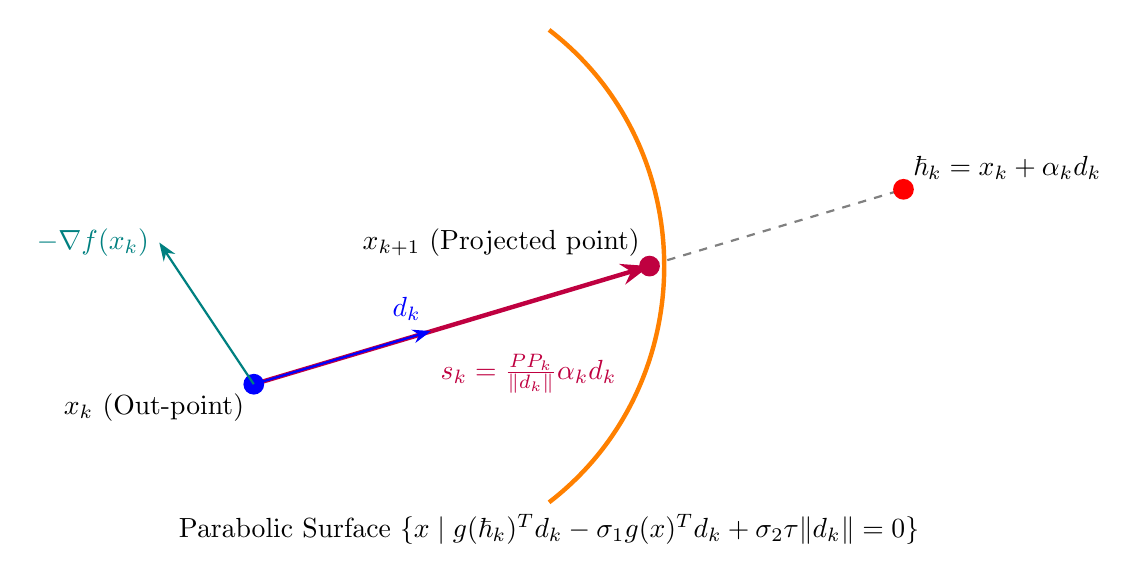
\begin{tikzpicture}[scale=1.5, >=Stealth]
		
		% 1. 绘制投影抛物面 (使用贝塞尔曲线模拟一个面对搜索方向的凸曲面)
		\draw[ultra thick, orange] (2.5, 3) .. controls (3.8, 2) and (3.8, 0) .. (2.5, -1) 
		node[below, text=black] {Parabolic Surface $\{x \mid g(\hbar_k)^T d_k - \sigma_1 g(x)^T d_k + \sigma_2 \tau \|d_k\| = 0\}$};
		
		% 2. 定义关键坐标点
		\coordinate (Xk) at (0, 0);                 % 当前迭代点
		\coordinate (Xk1) at (3.35, 1.0);           % 投影后的新点 (曲面上的交点)
		\coordinate (Hbar) at (5.5, 1.65);          % 初始线搜索的临时点 (越过了曲面)
		
		% 3. 绘制搜索方向的辅助虚线
		\draw[dashed, thick, gray] (Xk) -- (Hbar);
		
		% 4. 绘制实际更新的步长向量
		\draw[->, ultra thick, purple] (Xk) -- (Xk1);
		
		% 5. 绘制基础搜索方向 d_k
		\draw[->, thick, blue] (Xk) -- (1.5, 0.45) node[above left] {$d_k$};
		
		% 6. 添加数学公式标注
		\node[purple, below right, yshift=-5pt] at (1.5, 0.45) {$s_k = \frac{PP_k}{\|d_k\|} \alpha_k d_k$};
		
		% 7. 绘制点并添加文本标签
		\fill[blue] (Xk) circle (2.5pt) node[below left, text=black] {$x_k$ (Out-point)};
		\fill[purple] (Xk1) circle (2.5pt) node[above left, text=black] {$x_{k+1}$ (Projected point)};
		\fill[red] (Hbar) circle (2.5pt) node[above right, text=black] {$\hbar_k = x_k + \alpha_k d_k$};
		
		% 8. 绘制负梯度方向 (示意为何它是外点：与 d_k 夹角过大)
		\draw[->, thick, teal] (Xk) -- (-0.8, 1.2) node[left] {$-\nabla f(x_k)$};
		
	\end{tikzpicture}
\end{frame}

	\begin{frame}{Controlling $\|s_k\|$}
		\textbf{Standard DFP:} $s_k = \alpha_k d_k$ always.  
		If $g_k^\top d_k$ is very small, $\|s_k\|$ may grow very quickly. 
		
		\textbf{Projection DFP:}
		\begin{itemize}
			\item In-point: $g_k^\top d_k \le -\tau\|d_k\|$ $\Rightarrow$ $\|s_k\| \le \frac{1}{\tau}(-g_k^\top s_k)$.
			\item Out-point: Projection shortens the step: $\displaystyle \|s_k\| = \frac{PP_k}{\|d_k\|}\alpha_k\|d_k\|$ with $\frac{PP_k}{\|d_k\|}<1$.  
		Then we can prove that $PP_k \le -\sigma_3\, g_k^\top d_k$. 
			Hence $\|s_k\| \le -\sigma_3 \alpha_k g_k^\top d_k$.
		\end{itemize}
	\end{frame}
	
	\begin{frame}{Global Convergence of Projection DFP}
		So we can know that:
		\[
		\|s_k\| \le C \cdot (-\alpha_k g_k^\top d_k) \quad \text{for all }k,
		\]
		where $C = \max\{1/\tau,\ \sigma_3\}$.
		
		By Wolfe conditions, we can prove that
		\[
		\sum_{k=0}^{\infty} (-\alpha_k g_k^\top d_k) < \infty.
		\]
		Therefore
		\[
		\sum_{k=0}^{\infty} \|s_k\| < \infty.
		\]
		
		Hence the algorithm obviously converges globally.
	\end{frame}
	
\begin{frame}{Appendix}
\begin{figure}
	\centering
	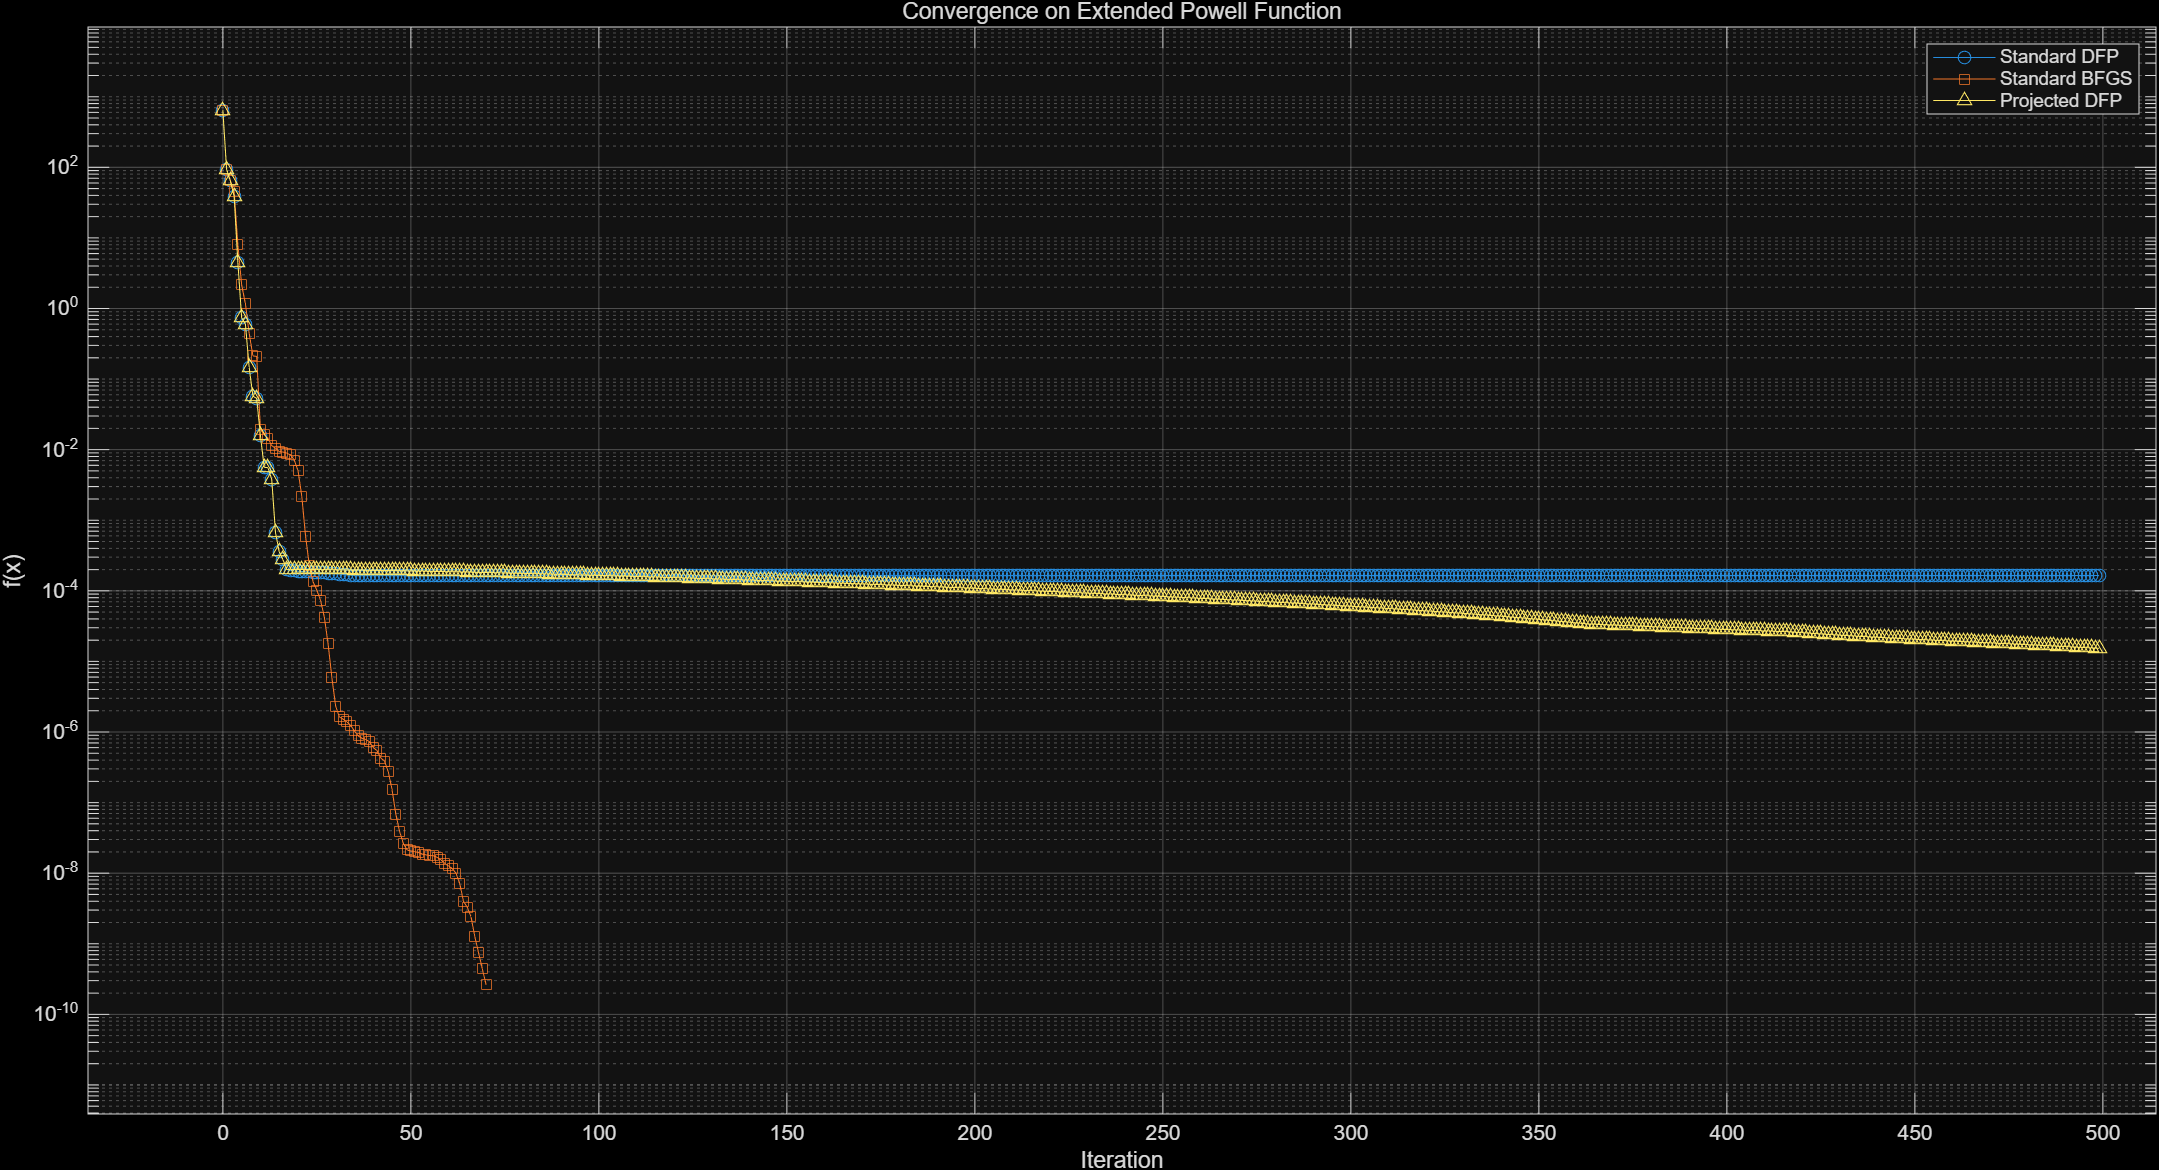
\includegraphics[width=0.7\linewidth]{comparison}
	\caption{Comparison experiment}
	\label{fig:comparison}
\end{figure}
\end{frame}
	\begin{frame}{References}
		\fontsize{6pt}{7pt}\selectfont
		\begin{thebibliography}{99}
			\bibitem{Davidon1991} W.~C. Davidon, \emph{Variable metric method for minimization}, SIAM J. Optim., 1(1):1–17, 1991.
			\bibitem{FletcherPowell1963} R.~Fletcher and M.~J.~D. Powell, \emph{A rapidly convergent descent method for minimization}, Comput. J., 6(2):163–168, 1963.
			\bibitem{Broyden1970} C.~G. Broyden, \emph{The convergence of a class of double-rank minimization algorithms}, J. Inst. Math. Appl., 6:76–90, 1970.
			\bibitem{Powell1971} M.~J.~D. Powell, \emph{On the convergence of the variable metric algorithm}, J. Inst. Math. Appl., 7:21–36, 1971.
			\bibitem{Powell1976} M.~J.~D. Powell, \emph{Some global convergence properties of a variable metric algorithm for minimization without exact line searches}, in Nonlinear Programming, SIAM-AMS Proceedings, Vol. IX, pp. 53–72, 1976.
			\bibitem{ByrdNocedalYuan1987} R.~H. Byrd, J.~Nocedal, Y.~Yuan, \emph{Global convergence of a class of quasi-Newton methods on convex problems}, SIAM J. Numer. Anal., 24:1171–1190, 1987.
			\bibitem{Yuan1995} Y.~Yuan, \emph{On the convergence of DFP algorithm}, Annals of Operations Research, 103:87–99, 2001 (Received 1995).
			\bibitem{YuanZhouPham2026} G.~Yuan, P.~Zhou, H.~T.~Pham, \emph{A projection DFP quasi-Newton algorithm and its applications}, Numerical Algorithms, 2026.
		\end{thebibliography}
	\end{frame}
	\begin{frame}{Thank you!}
		\centering \Huge Thanks for your attention! \\[1cm]
		\Large Questions?
	\end{frame}
\end{document}